\makeatletter \@ifundefined{rootpath}{\input{../../setup/preamble.tex}}\makeatother
\worksheetstart{Roslyn}{0}{Februar 10, 2015}{}{../../}
This chapter presents a conceptual overview of the Roslyn project. In BLA we describe BLA\toby{Ændre dette når vi ved hvad der skal være i kapitlet}

\section{Introduction}
Project Roslyn is Microsoft's initiative of completely rewriting the C\# and \ac{VB} compilers, using their own managed code language. That is, the C\# compiler is written in C\# and the \ac{VB} compiler in \ac{VB}. Roslyn was released open source at the Microsoft Build Conference 2014\cite{csharpBuild}.

Beyond changing the languages the compilers are written in, Roslyn provides a new approach to compiler interaction and usage. Traditionally a compiler is treated as a black box where it is given some source files as input, magic happens in the middle, and out comes objects files or assemblies\cite[p. 3]{ng2012roslyn}. During compilation the compiler builds a deep knowledge about the code, unavailable to the programmer, which is discarded once the compilation is done. This is where Roslyn differs, as it exposes the code analysis of the compiler by providing an API layer, which allows the programmer to obtain information about the different compilation phases\cite[p. 3]{ng2012roslyn}. 

The compiler APIs available are illustrated in \bsref{fig:api_vs_compiler_pipeline} where each API corresponds to a phase in the compiler pipeline. In the first phase the source code is turned into tokens and parsed according to the language grammar. This phase is exposed through an API as a syntax tree. In the second phase declarations i.e. namespaces and types from code and imported metadata are analyzed to form named symbols. This phase is exposed as a hierarchical symbol table. In the third phase identifiers in the code are matched to symbols.\toby{Det inkluderer type check og scope check også?} This phase is exposed as a model which exposes the result of the semantic analysis. In the last phase, information gathered throughout compilation is used to emit an assembly. This phase is exposed as an API that produces IL byte code\cite[p. 3-4]{ng2012roslyn}.
%second phase:  a kind of an index to the sources that tells where namespaces and types are declared

\begin{figure}[htbp]
\centering
 \includegraphics[width=1\textwidth]{\rootpath/worksheets/roslyn/figures/compiler_pipeline_vs_api} 
 \caption{Compiler pipeline in contrast to compiler APIs\cite[p. 4]{ng2012roslyn}.}
\label{fig:api_vs_compiler_pipeline}
\end{figure}

Knowledge obtained through the APIs can be valuable in order to create tools that analyze and transform C\# or \ac{VB} code. Furthermore Roslyn allows interactive use of the languages using a \acs{REPL}\footnote{http://blogs.msdn.com/b/csharpfaq/archive/2012/01/30/roslyn-ctp-introduces-interactive-code-for-c.aspx}, and embedding of  C\# and \ac{VB} in a \ac{DSL}\cite[p. 3]{ng2012roslyn}.

\section{Inside Roslyn}
In this section we will describe the inner architecture of Roslyn's source code and further elaborate on the compiler phases from \bsref{fig:api_vs_compiler_pipeline}.

\begin{figure}[htbp]
\centering
 \includegraphics[width=0.4\textwidth]{\rootpath/worksheets/roslyn/figures/roslyn_solution_overview} 
 \caption{Overview of projects in Roslyn solution.}
\label{fig:roslyn_solution_overview}
\end{figure}

The Roslyn solution available on github\footnote{https://github.com/dotnet/roslyn}, forked on the 9th February 2015, consists of 118 projects which include projects for Visual Studio development, interactive usage of the languages and more as illustrated on \bsref{fig:roslyn_solution_overview}. We will focus on the \bscode{Compilers} folder which contains the source code for the C\# and \ac{VB} compiler, each located in a separate folder. They share common code and functionality within the \bscode{Core} folder which includes code for controlling the overall compilation flow. We describe only the C\# compiler and the core code. However, the code for each compiler is very similar and use the same patterns for compilation\cite[09:36-10:36]{campbellDeeperRos}, so most of the following will apply for the \ac{VB} compiler also.

\begin{figure}[htbp]
\centering
 \includegraphics[width=0.4\textwidth]{\rootpath/worksheets/roslyn/figures/roslyn_csharp_overview} 
 \caption{Overview of CSharp folder.}
\label{fig:roslyn_csharp_overview}
\end{figure}

The projects contained in the \bscode{CSharp} folder are shown on \bsref{fig:roslyn_csharp_overview}. The important projects are \bscode{csc}, \bscode{CSharpCodeAnalysis.Portable} and \bscode{CSharpCodeAnalysis.Desktop}. The \bscode{csc} project is the C\# command line compiler, which is the starting point of a C\# compilation. The two other projects contain the actual code required for compilation. The rest of the projects in the \bscode{CSharp} folder mainly involves tests for the C\# compiler.

In \bsref{fig:roslyn_invoke_overview} an overview of the compilation call chain is shown. Compilation starts with \bscode{csc's} main method being invoked, which calls the static \bscode{Run} method on the \bscode{Csc} class. This method creates a new \bscode{compiler} object of type \bscode{Csc}. \bscode{Csc} is a subtype of \bscode{CSharpCompiler}, located in the \bscode{CSharp.CSharpCodeAnalysis.Desktop} project, which again is a subtype of \bscode{CommonCompiler}, located in \bscode{Core.CodeAnalysis}. This means that the creation of the \bscode{compiler} object, calls the constructors of \bscode{Csc}, \bscode{CSharpCompiler} and \bscode{CommonCompiler}. Afterwards the \bscode{Run} method is invoked on the \bscode{compiler} object, which further invokes its parents \bscode{Run} method, which again invokes its parent \bscode{Run} method. Finally the \bscode{RunCore} method in \bscode{CommonCompiler} is invoked, which contains the general code that controls the overall flow of the compiler pipeline, that was illustrated in \bsref{fig:api_vs_compiler_pipeline}. The \bscode{RunCore} method will for the phases at run time call the actual compiler logic for C\# in \bscode{CSharp.CSharpCodeAnalysis.Portable} or \ac{VB} in \bscode{VisualBasic.BasicCodeAnalysis.Portable} through dynamic dispatch.\toby{Er det helt rigtigt? Muligvis kalder den også i noget generelt, som kun er defineret i core, der ikke kalder videre. Tror måske IL emitting, kun har kode i Core - men er også noget i CSharpCodeAnalysis med kodegenerering. Andet eksempel: SemanticModel ligger i Core.}

\begin{sidewaysfigure}[htbp]
\centering
 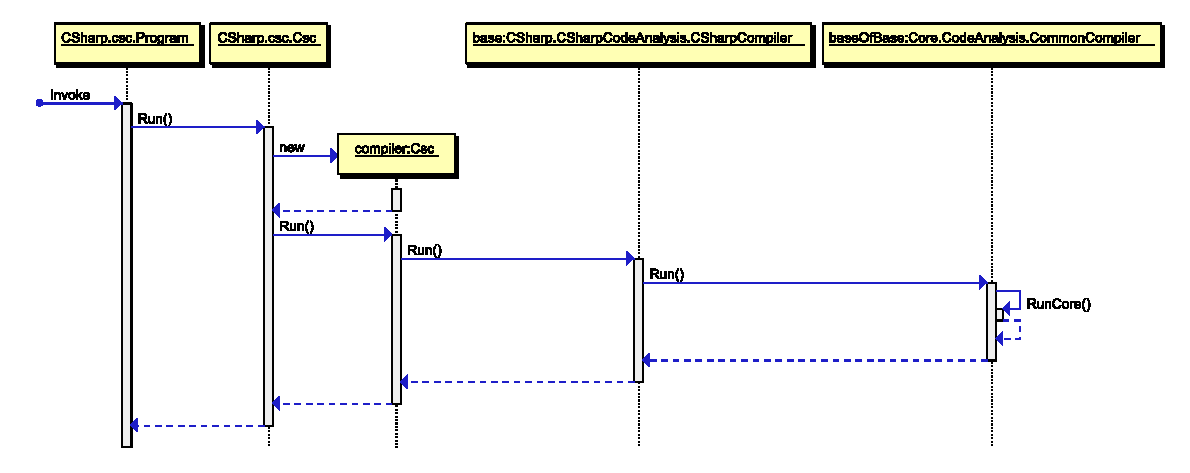
\includegraphics[width=\textwidth]{\rootpath/worksheets/roslyn/figures/seq_diagrams/roslyn_invoke_overview} 
 \caption{Sequence diagram showing an overview of the call chain of a C\# compilation.}
\label{fig:roslyn_invoke_overview}
\end{sidewaysfigure}

\subsection{CSharpCodeAnalysis}
%fortæl om CSharpCodeAnalysis projekterne

\begin{figure}[htbp]
\centering
 \includegraphics[width=0.4\textwidth]{\rootpath/worksheets/roslyn/figures/csharp_codeanalysis_overview} 
 \caption{Overview of the \bscode{CSharp.CSharpCodeAnalysis.Portable} project.}
\label{fig:roslyn_csharpanalysis_overview}
\end{figure}
\toby[i]{Ved ikke om jeg vil have den her figur med}

\section{Key Concepts}
The C\# compiler builds upon concepts from traditional compiler theory, such as lexing, parsing, declaration processing, semantic analysis and code generation\cite{sebestaProLang}\cite{fischer2009crafting}. Throughout the phases of compilation, traditional concepts such as a syntax tree, symbol table and visitor pattern are also used. In this section we describe the core concepts used in the C\# compilation phases.

\toby[i]{Måske inddel i syntax og semantic subsubsektioner (dem under)}

\subsection{Syntax trees}
Syntax trees are the primary structure used throughout the phases of compilation. Roslyn's syntax tress have three key attributes\cite[p. 6]{ng2012roslyn}. The first attribute is that a syntax tree is a \textit{full fidelity} representation of source code, which means that everything in the source code is represented as a node in the syntax tree. If programs are invalid, the syntax tree represent these errors in source code by skipped or missing tokens in the tree. 

The first attribute enables the second attribute, which is that a syntax tree produced from parsing must be \textit{round-trippable} back to the original source code.

The third attribute is that syntax trees are immutable and thread-safe. This enables multiple users to use the same syntax tree at the same time in different threads without concurrency issues. As syntax trees are immutable, factory methods exists in order to help create and modify trees. This might seem inefficient, as one would expect a copy of the tree is required, however syntax tress are efficient as they reuse underlying nodes. This means trees can be modified fast and with a low memory overhead.

In fact there exists two types of tress in Roslyn, which we will describe.
%fortæl måske først om det nede i røde og grønne træer

 at least for one kind of tree

%trees are efficient in the way they reuse underlying nodes, so the new version can be rebuilt fast and with little extra memory.

%A syntax tree is literally a tree data structure, where non-terminal structural elements parent other elements. Each syntax tree is made up of nodes, tokens, and trivia.



 which means that a tree never changes

This enables

Meaning that a tree is never changed 

\subsubsection{Red And Green Trees}
%syntax træ generelt.
%røde og grønne træer

\toby[i]{Måske skal nogen af disse op foran træet}
\subsection{Syntax Nodes}
\subsection{Syntax Tokens}
\subsection{Syntax Trivia}
\subsection{Spans}
\subsection{Kinds}
\subsection{Errors}

\subsection{Compilation}
\subsection{Symbols}



%ng2012roslyn
\section{Compile Phases}\toby{tror den her titel skal slettes nu (bliver fortalt i intro og inside roslyn istedet}
\toby[i]{Skal have det et sted, hvor jeg fortæller mere præcist en compiler line billedet om faserne der sker, ligesom beskrevet i blogpostet. Også i forhold til om de køres med en eller flere tråde}
%Earlier in intro we looked at the phases of the compiler in contrast to the compiler API, howerver This does not include all phases. In this section we will explain in more detail what phases the compiler consits of and how it is build on in the code
	%Omformuler så det lyder bedere (men noget i den stil)

%Forklar de forskellige kompilerigns faser

%overordnet beskrivelse af faserne og evt. hvis api i forhold til også
	%ved ikke om jeg skal bruges deres tegning eller lave en ny selv (eller begge dele)

%snak ikke om det under white paper underskriften: API Layers

\section{Core Concepts}
%syntax tree, syntax tokens, symbols osv.

%MORE:

%Known Limitations and Unimplemented Language Features
	%https://social.msdn.microsoft.com/Forums/vstudio/en-US/f5adeaf0-49d0-42dc-861b-0f6ffd731825/known-limitations-and-unimplemented-language-features?forum=roslyn

%Liste over mulige emner:
	% Beskrivelse af kompileren, og hvad de muliggøre med deres API.
	% De enkelte faser i kompileren og generelt om dens opbygning
	% Hvilke ting de har gjort i forhold til at forbedre performance
	% Fortælle om deres røde og grønne syntaks træ
	% De anvender traditionel compiler teori, med lexer og parser + syntaxtræ og visitor til at traverserer træet. og emit fase.
	%Evt. fortæl om faserne i forhold til mapperne i projektet. Med Core, VB og C# projekternere og til sidst fortæl udfra C#'s mapper (og de forskellige faser).
	%Evt. også nævn syntax visualizer (nok ikke så vigtig, men er et værdifuldt værktøj)
	%Immutable data struktuerer!
	%Hvilke muligheder man har for at implementere STM direkte i Roslyn
		%Ved hjælp af API, hvor vi gør det først og derefter fodrer output til csc.exe
		%Direkte i compileren.


%Den primære brug der er tiltænkt at programmøren skal få adgang er gennem API laget, hvor en del kompleksitet stadig er gemt væk.
	%Vi vil gå direkte ind og ændre i selve compileren, hvilket ikke er tiltænk som hovedtanken fra Microsoft's side.
\worksheetend